\chapter{Населённые пункты}
\label{ch:human-settlement}

	Викиданные представляют собой базу структурированных данных. В статье исследуется объект Викиданных <<населённый пункт>> (human settlement) и его свойства. 
В каждом из разделов представлены задачи, решённые с помощью SPARQL-запросов. В их числе: нахождение экземпляров объекта <<населённый пункт>>, построение
упорядоченного списка стран по суммарному количеству населения, проживающего в <<населённых пунктах>>, и списка объектов, сопутствующих <<населённым 
пунктам>> в свойстве <<экземпляр>> (instance of). Также построена диаграмма, показывающая долю населения страны, проживающего в <<населённых пунктах>>. 
Диаграмма показывает, что высокий процент населения, проживающего в <<населённых пунктах>>, приходится на менее промышленные страны, в то время как в более 
индустриальных странах меньшая доля населения проживает в <<населённых пунктах>>. На 2017 год Википедия описывает примерно половину населённых пунктов 
(75 тыс.), Викиданные содержат менее 3\% таких поселений (4 тыс.) относительно данных переписи за 2010 год (155,5 тыс.). Для улучшения результатов решения 
вышеописанных задач находили более общие объекты и указывали их в исследуемом объекте с помощью свойства <<экземляр>> (instance of). Трудность исследования 
вызвана отсутствием чёткой типологии населённых пунктов (например, от численности населения) в законодательстве России и в Викиданных.

%%%%
\section{Экземпляры объекта <<Населённый пункт>>}

Для построения списка всех населённых пунктов нам потребуются объект 
\wdqName{<<Населённый пункт>>}{486972} и свойство \wdProperty{31}{<<экземпляры>>} 
(листинг ~\protect\ref{lst:human-settlement1}).

\begin{lstlisting}[ language=SPARQL, 
                    caption={\href{https://w.wiki/49WB}{Список всех Населённых пунктов}\protect\footnotemark},
                    label=lst:human-settlement1,
                    texcl 
                    ]
# List of all human settlements
SELECT ?hum ?humLabel 
WHERE 
{
  ?hum wdt:P31 wd:Q486972. # instance of human settlement  
  SERVICE wikibase:label { bd:serviceParam wikibase:language 
							"ru,[AUTO_LANGUAGE]"}
}
\end{lstlisting}%
\footnotetext{Получено \num{411393} записи в 2017 году.  Ссылка на SPARQL-запрос: \href{https://w.wiki/49WB}{https://w.wiki/49WB}}

В 2021 году список населённых пунктов получить невозможно из-за большого числа объектов и поэтому слишком долгой работы скрипта. Произведем подсчёт всех населённых пунктов (листинг ~\protect\ref{lst:human-settlement2}).

\begin{lstlisting}[ language=SPARQL, 
                    caption={\href{https://w.wiki/49WC}{Количество всех Населённых пунктов}\protect\footnotemark},
                    label=lst:human-settlement2,
                    texcl 
                    ]
# Number of human settlements
SELECT (COUNT(?hum) AS ?count) 
WHERE {
  ?hum wdt:P31 wd:Q486972. # instance of human settlement  
  SERVICE wikibase:label { bd:serviceParam wikibase:language 
							"ru,[AUTO_LANGUAGE]"}
}
\end{lstlisting}%
\footnotetext{Получено \num{563126} записи в 2021 году. Ссылка на SPARQL-запрос: \href{https://w.wiki/49WC}{https://w.wiki/49WC}}

Наиболее полными и проработанными населёнными пунктами на Викиданных являются:  \href{http://www.wikidata.org/entity/Q80561}{Антакья}, \href{http://www.wikidata.org/entity/Q52506}{Хенераль Рока}, \href{http://www.wikidata.org/entity/Q51063}{Падре Лас Касас}.

Почти пустыми и малоинформативными населёнными пунктами оказались: \href{http://www.wikidata.org/entity/Q31913786}{Беломорск}, \href{http://www.wikidata.org/entity/Q37958167}{Сегежа}, \href{http://www.wikidata.org/entity/Q33522990}{Янишполе}.

Произведено объединение дублей объектов \href{http://www.wikidata.org/entity/Q31913786}{Беломорск} с \href{http://www.wikidata.org/entity/Q104773}{Беломорск}, \href{http://www.wikidata.org/entity/Q37958167}{Сегежа} с \href{http://www.wikidata.org/entity/Q193922}{Сегежа}, \href{http://www.wikidata.org/entity/Q33522990}{Янишполе} с \href{http://www.wikidata.org/entity/Q16024734}{Янишполе}.

Среди отечественных населённых пунктов в Викиданных больше всего свойств по данным ProWD у \href{http://www.wikidata.org/entity/Q128499}{Ялты} (\num{36} свойств). Лидером по всему миру является \href{http://www.wikidata.org/entity/Q1490}{Токио} (\num{73} свойства). \protect\footnotemark

\footnotetext{По данным ProWD: \href{https://prowd.id/dashboards/f64fc6d3d55d/profile}{https://prowd.id/dashboards/f64fc6d3d55d/profile}}


%%%%
\section{Список стран по суммарному количеству населения}

Построим упорядоченный список стран по суммарному количеству населения, проживающего в <<населённых пунктах>> (листинг ~\protect\ref{lst:human-settlement3}).

\begin{lstlisting}[ language=SPARQL, 
                    caption={\href{https://w.wiki/49W2}{Список стран по суммарному количеству населения}\protect\footnotemark},
                    label=lst:human-settlement3,
                    texcl 
                    ]
# List of countries by population in settlements
SELECT ?country ?countryLabel (SUM(?population) as ?sumPopulation)
WHERE
{
  ?hum wdt:P31 wd:Q486972; # instance of human settlement
       wdt:P17 ?country;   # settlement in the ?country
       wdt:P1082 ?population. # settlement has ?population
  
  SERVICE wikibase:label { bd:serviceParam wikibase:language 
						"ru,[AUTO_LANGUAGE]"}
}
GROUP BY ?country ?countryLabel 
ORDER BY DESC (?sumPopulation)
\end{lstlisting}%
\footnotetext{Получено \num{161} запись в 2017 году и \num{213} записей в 2021 году. Ссылка на SPARQL-запрос: \href{https://w.wiki/49W2}{https://w.wiki/49W2}}

Для группирования населённых пунктов по странам, используем команду GROUP BY в предпоследней строчке скрипта выше.

Пузырьковая диаграмма ниже показывает соотношение стран по количеству населения в <<населённых пунктах>>.

\begin{figure}
\centering
	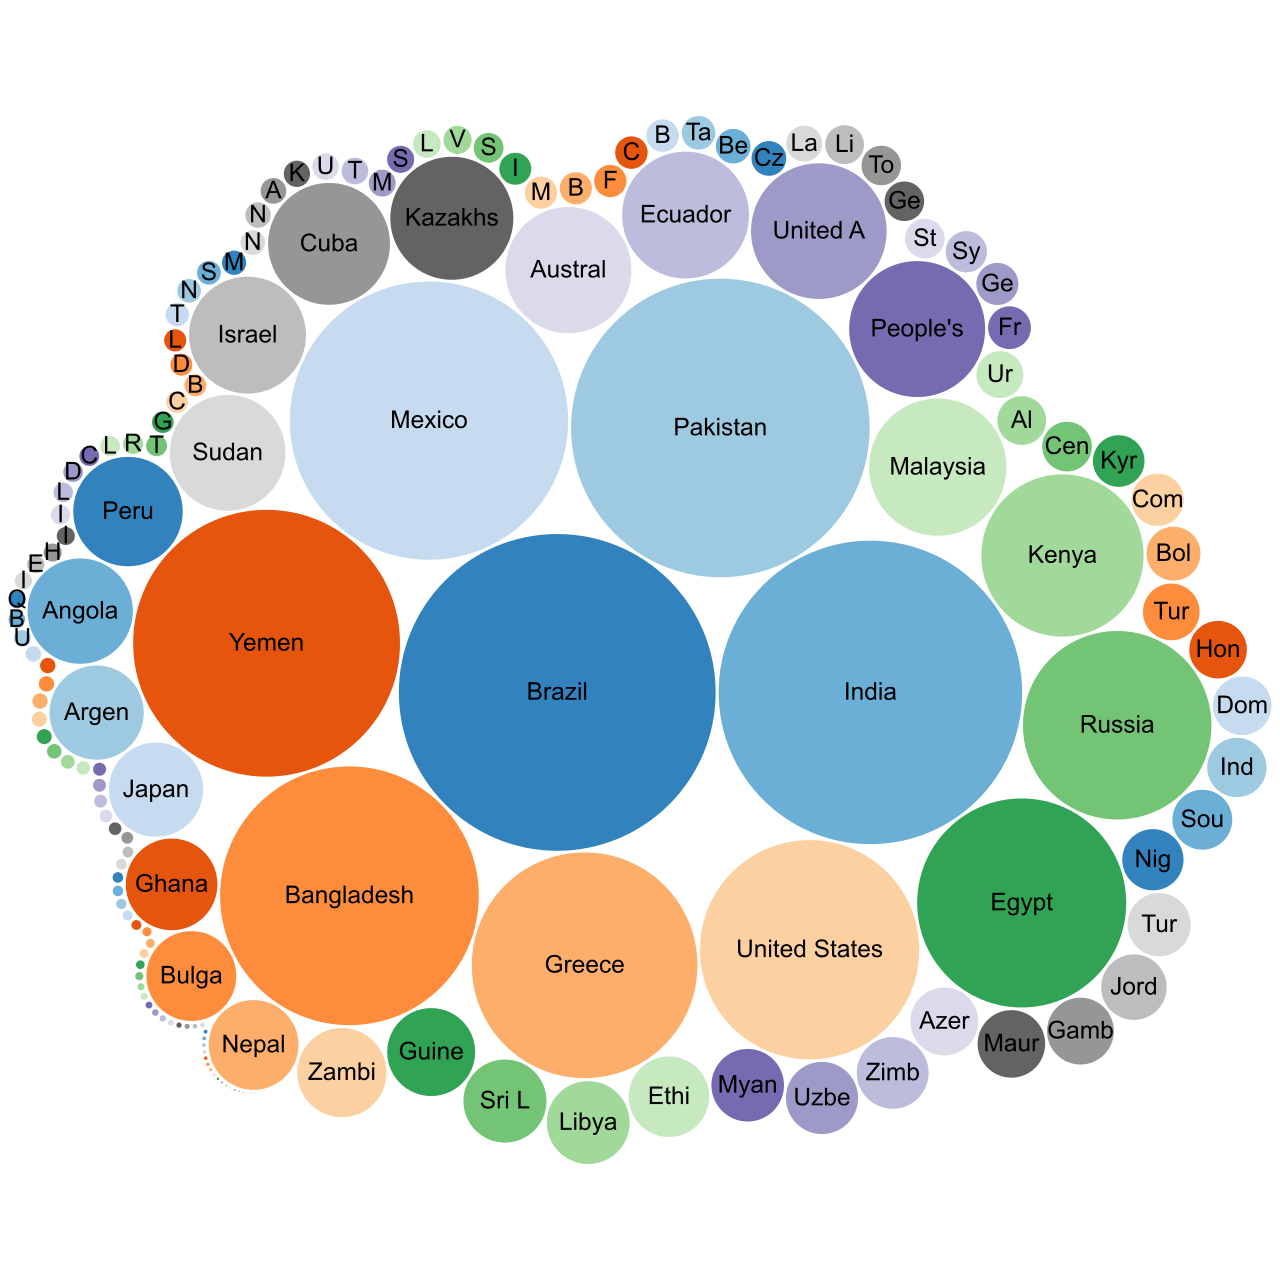
\includegraphics[width=0.9\linewidth]{./chapter/human_settlement/AnnaBubbleHumanSettlement.jpg}
	\label{fig:human-settlement-1}
    \caption[Пузырьковая диаграмма  по суммарному количеству населения в населённых пунктах, 2017.]{Пузырьковая диаграмма  по суммарному количеству населения, проживающего в объектах типа <<населённый пункт>> на 2017 год. Размер пузырька соответствует числу населения для одной страны. Ссылка на SPARQL-запрос: \href{https://w.wiki/49W2}{https://w.wiki/49W2}}
\end{figure}

\begin{figure}
\centering
	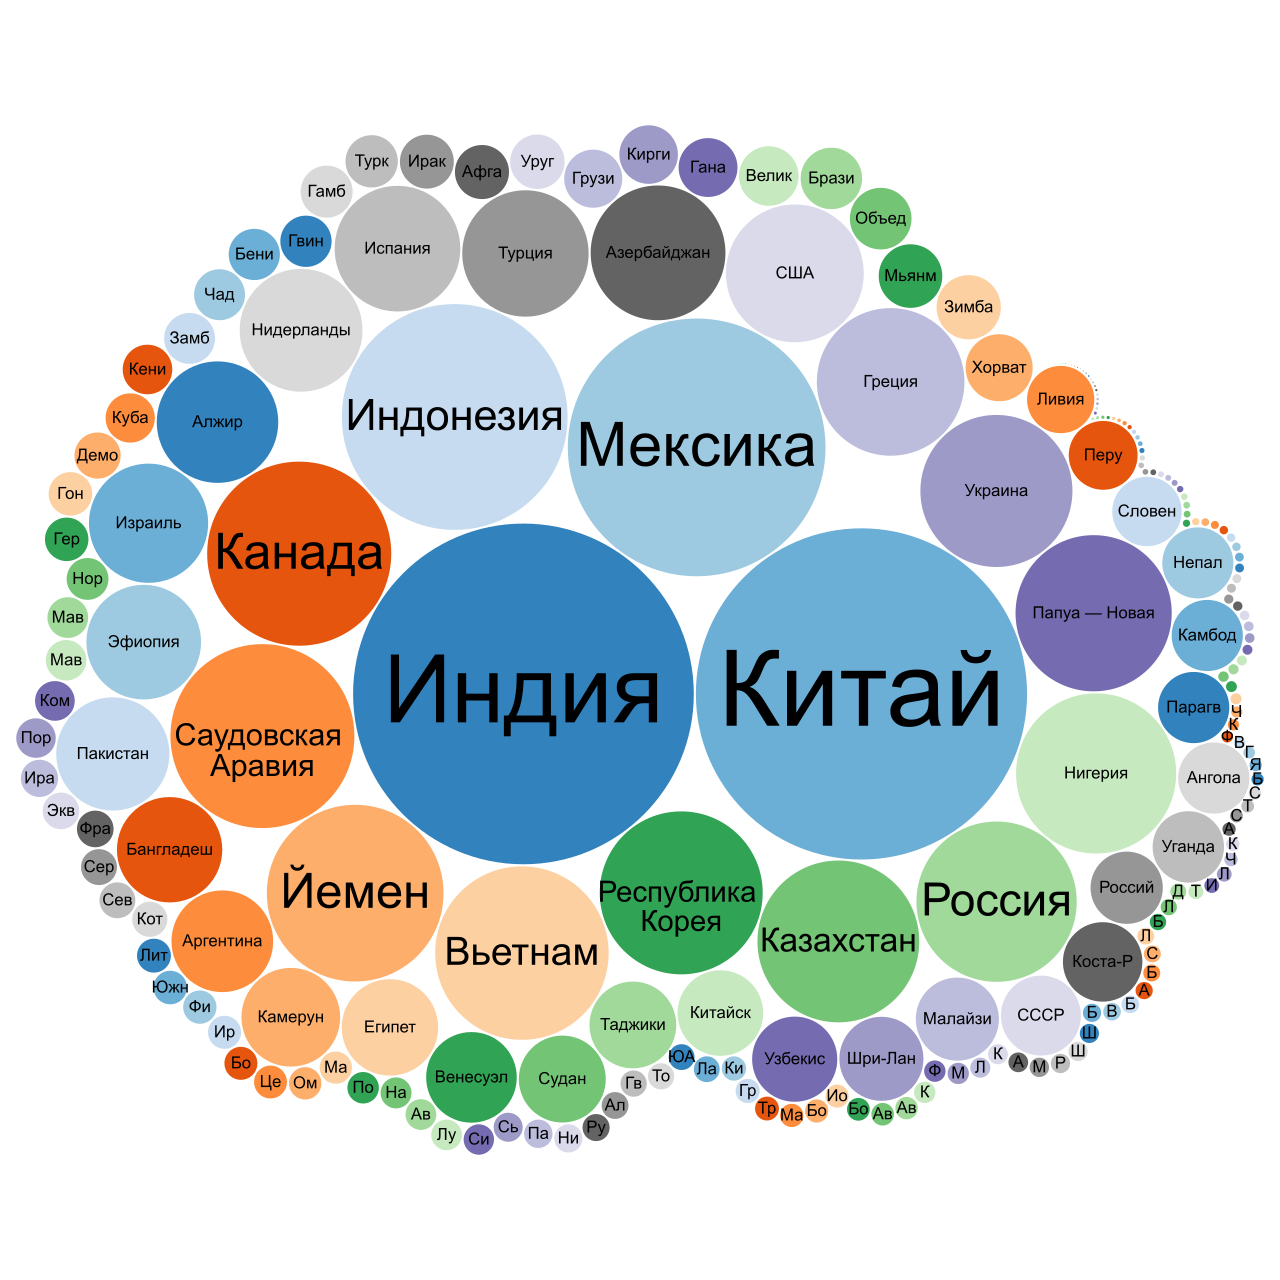
\includegraphics[width=0.9\linewidth]{./chapter/human_settlement/LeonidBubbleHumanSettlement.jpg}
	\label{fig:human-settlement-2}
	\caption[Пузырьковая диаграмма  по суммарному количеству населения в населённых пунктах, 2021.]{Пузырьковая диаграмма  по суммарному количеству населения, проживающего в объектах типа <<населённый пункт>> на 2021 год. Размер пузырька соответствует числу населения для одной страны. Ссылка на SPARQL-запрос: \href{https://w.wiki/49W2}{https://w.wiki/49W2}}
\end{figure}

Результаты запросов в 2017 и 2021 имеют сильно разные результаты. В 2017 году большее количество населения проживало в объектах <<населённый пункт>> в таких странах, как: \href{http://www.wikidata.org/entity/Q155}{Бразилия} (\num{12} млн), \href{http://www.wikidata.org/entity/Q843}{Пакистан} (\num{10} млн), \href{http://www.wikidata.org/entity/Q96}{Мексика} (\num{8} млн), \href{http://www.wikidata.org/entity/Q805}{Йемен} (\num{8} млн), \href{http://www.wikidata.org/entity/Q668}{Индия} (\num{7} млн), \href{http://www.wikidata.org/entity/Q902}{Бангладеш} (\num{7} млн). Эти страны имеют пригодные климатические и географические условия для комфортного проживания относительно небольших населённых пунктах. Однако в 2021 году список значительно изменился: \href{http://www.wikidata.org/entity/Q668}{Индия} (\num{30} млн), \href{http://www.wikidata.org/entity/Q148}{Китай} (\num{28} млн), \href{http://www.wikidata.org/entity/Q96}{Мексика} (\num{17} млн), \href{http://www.wikidata.org/entity/Q252}{Индонезия} (\num{13} млн), \href{http://www.wikidata.org/entity/Q16}{Канада} (\num{9} млн), \href{http://www.wikidata.org/entity/Q851}{Саудовская Аравия} (\num{9} млн).


%%%%%
\subsection{Проверка правильности выполнения скрипта}

Проверим правильность подсчётов вышеописанного запроса, который строит список стран по суммарному числу населения. Для этого напишем скрипт~---  \href{https://w.wiki/4CzZ}{SPARQL-запрос}, где для самой малолюдной страны будет построен список поселений с количеством их жителей. В 2017 году запрос показал, что такой страной является \href{http://www.wikidata.org/entity/Q236}{Черногория}. В 2021 году такой страной является \href{http://www.wikidata.org/entity/Q760}{Сент-Люсия}. Немного изменим тот же скрипт и выведем число жителей населённых пунктов \href{http://www.wikidata.org/entity/Q760}{Сент-Люсия}.

\begin{lstlisting}[ language=SPARQL, 
                    caption={\href{https://w.wiki/4Cza}{Список стран по суммарному количеству населения}\protect\footnotemark},
                    label=lst:human-settlement4,
                    texcl 
                    ]
# Population in settlements in the Saint Lucia 
SELECT (sum(?population) as ?total)
WHERE {
  ?hum wdt:P31 wd:Q486972.    # instance of human settlement
  ?hum wdt:P17 wd:Q760.       # settlement in the Saint Lucia
  ?hum wdt:P1082 ?population. # settlement has ?population
  SERVICE wikibase:label { bd:serviceParam wikibase:language 
				"ru,[AUTO_LANGUAGE]"}
 }
\end{lstlisting}%
\footnotetext{Проверка прошла успешно, так как данный скрипт подтвердил результат численности населения, проживающего в <<населённых пунктах>> \href{http://www.wikidata.org/entity/Q760}{Сент-Люсия}. Ссылка на SPARQL-запрос: \href{https://w.wiki/4Cza}{https://w.wiki/4Cza}}

%%%%%
\subsection{Полнота Викиданных}

Населённый пункт — это общее название мест с постоянными жителями \protect\footnotemark. \footnotetext{Ожегов С. И. Толковый словарь русского языка, 2003} По версии редакторов Викиданных в понятие насёленный пункт входят города, сёла, деревни и другие. Полный список можно увидеть в разделе этой статьи «Cписок объектов, сопутствующих "human\_settlement" в "instance of"». Точной информации о количестве населённых пунктов в мире не было найдено. Поэтому проверим полноту населённых пунктов, которые есть в Викиданных и которые использовались для решения задачи. Была поставлена задача: построить упорядоченный список стран по суммарному количеству населения, проживающего в \href{http://www.wikidata.org/entity/Q486972}{населённых пунктах}. Для этого напишем \href{https://w.wiki/4FUz}{SPARQL-запрос} \protect\footnotemark, который выведет населённые пункты с незаполненным свойством \href{http://www.wikidata.org/entity/P1082}{численность населения}. 
\footnotetext{ В 2017 году этот запрос выдал \num{372997} таких населённых пунктов. Произведя расчеты получаем, что только у \num{9,3}\% населенных пунктов мира указано количество населения (свойство 'population'). Проводя ту же проверку в 2021 году, запрос выдал \num{507078} таких населённых пунктов. Получаем \num{11,2}\% населенных пунктов мира имеют свойство 'population'.} 
А теперь посмотрим населённые пункты, у которых не указана принадлежность к какой-либо стране~--- \href{https://w.wiki/4FV8}{SPARQL-запрос}\protect\footnotemark.

\footnotetext{В 2017 году таких нашлось \num{8427} объектов. В 2021 году таких объектов уже существенно больше - \num{27824}. Поэтому в результате решения данной задачи получились неполная картина о суммарном количестве населения в населённых пунктах по странам.}

Рассмотрим населённые пункты России. По данным проекта "Населённые пункты России/Статистика" Русская Википедия содержит приблизительно 75000 статей о населённых пунктах России. По переписи 2010 года в России 155 510 населённых пунктов. Проверим, сколько объектов содержится в Викиданных о населённых пунктах России с помощью следующего \href{https://w.wiki/4FVE}{SPARQL-запроса}\protect\footnotemark. 

\footnotetext{В 2017 году было получено \num{4113} объектов, что составляет \num{2,6}\% от общего числа населённых пунктов по переписи за 2010 год. В 2021 году запрос выдал \num{17425} объектов, что составляет \num{11,2}\% от общего числа населённых пунктов. Таким образом, в Викиданных содержится слишком мало информации о населённых пунктах России.}

Итак, степень заполненности Викиданных по населённым пунктам низкая. А именно, у некоторых городов, поселков, деревень и других населённых пунктов на Викиданны отсутствует свойство \href{http://www.wikidata.org/entity/Q21503252}{экземпляр}, значением которого может быть \href{http://www.wikidata.org/entity/Q486972}{населённый пункт}. Кроме того, есть почти пустые и плохо проработанные объекты. Для решения этих проблем необходимо заполнять эти свойства и связывать между собой объекты Викиданных.

%%%%%
\subsection{Заполнение Викиданных}

В ходе заполнения объектов Викиданных было решено заполнять свойство \href{http://www.wikidata.org/entity/Q21503252}{экземпляр}.

Были внесены данные о \num{100} объектах России, которые не имели значения \href{http://www.wikidata.org/entity/Q486972}{населённый пункт} в свойстве \href{http://www.wikidata.org/entity/Q21503252}{экземпляр}.

На 25.10.2017, после заполнения данными, Викиданные содержали \num{4207} объектов о населённых пунктах России, что составляло \num{2,6}\% от общего числа населённых пунктов по переписи за 2010 год и \num{5,6}\% от данных Русской Википедии. Это можно увидеть с помощью следующего \href{https://w.wiki/4FVE}{SPARQL-запроса}.

%%%%%
\section{Доля населения страны, проживающего в <<human\_settlement>>}

Построим упорядоченный список стран доли населения (в процентах), проживающего в \href{http://www.wikidata.org/entity/Q486972}{населённых пунктах}, к числу всех жителей страны.

\begin{lstlisting}[ language=SPARQL, 
                    caption={\href{https://w.wiki/4Cza}{соотношение количества людей, проживающих в селе, к количеству людей, проживающих в стране.}\protect\footnotemark},
                    label=lst:human-settlement5,
                    texcl 
                    ]
# An ordered list of the ratio of the number of people living in 
"settlement" to the number of inhabitants in the country.
SELECT ?countryLabel (SUM(?population / ?pop) 
	as ?proportionPopulation) (?proportionPopulation
	 * 100 as ?percentPopulation)
WHERE {
  ?hum wdt:P31 wd:Q486972.    # instances of human settlement  
  ?hum wdt:P17 ?country.      # country 
  ?hum wdt:P1082 ?population. # population
  ?country wdt:P1082 ?pop.    # population in the country
  SERVICE wikibase:label { bd:serviceParam wikibase:language 
	"ru,[AUTO_LANGUAGE]"}
  }
GROUP BY ?country ?countryLabel
ORDER BY DESC (?percentPopulation)
\end{lstlisting}%
\footnotetext{Получено \num{158} записей в 2017 году и \num{206} записей в 2021 году. \href{https://w.wiki/4T4s}{Ссылка.}}

Столбчатая диаграмма на рисунке позволяет увидеть для каждой отдельной страны отношение количества людей, проживающих в \href{http://www.wikidata.org/entity/Q486972}{населённых пунктах} к числу жителей в стране.

\begin{figure*}
    \setlength{\fboxsep}{0pt}%
    \setlength{\fboxrule}{1pt}%
    \fcolorbox{gray}{gray}{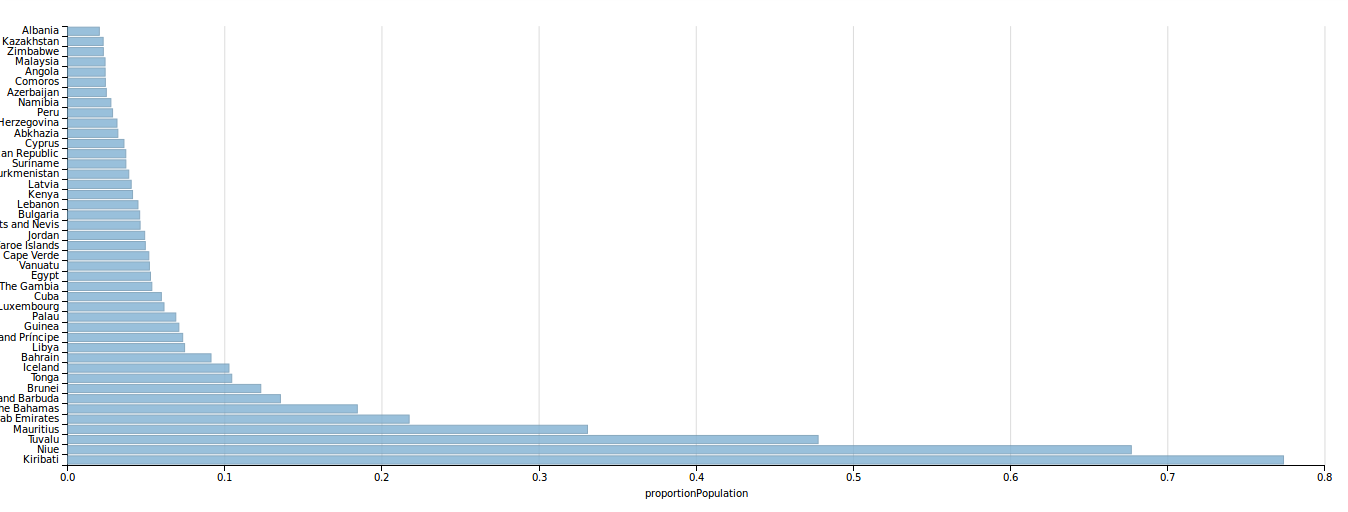
\includegraphics[width=0.9\linewidth]{./chapter/human_settlement/AnnaShareHumanSettlement.png}}
	\label{fig:human-settlement-3}
	\caption[Диаграмма доли населения страны. Карелия, 2017.]{Диаграмма доли населения страны, проживающего в "населённых пунктах" (2017). Ссылка на SPARQL-запрос: \href{https://w.wiki/4T4s}{https://w.wiki/4T4s}.}%
\end{figure*} 

\begin{figure*}
    \setlength{\fboxsep}{0pt}%
    \setlength{\fboxrule}{1pt}%
    \fcolorbox{gray}{gray}{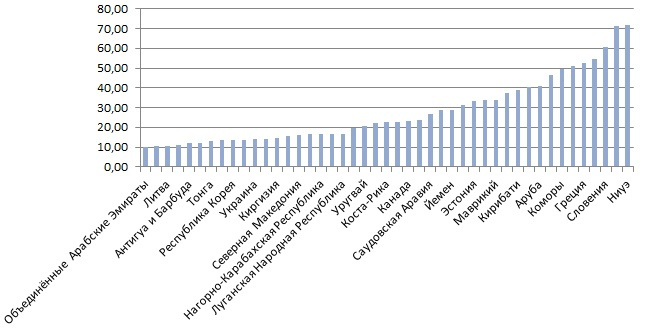
\includegraphics[width=0.9\linewidth]{./chapter/human_settlement/LeonidShareHumanSettlement.jpg}}
	\label{fig:human-settlement-4}
	\caption[Диаграмма доли населения страны, 2021.]{Диаграмма доли населения страны, проживающего в "населённых пунктах" (2021). Ссылка на SPARQL-запрос: \href{https://w.wiki/4T4s}{https://w.wiki/4T4s}.}%
\end{figure*} 

Из графика видно, что наиболее высокий процент в 2017 году приходился на следующие страны: Кирибати (78\%), Ниуэ (70\%), Греция (53\%), Тувалу (48\%), Коморы (43\%), Маврикий (42\%). В 2021 году ситуация полностью поменялась: Ниуэ (72\%), Папуа — Новая Гвинея (71\%), Словения (61\%), Фарерские острова (54\%), Греция (53\%), Маршалловы Острова (51\%). Интересно заметить, что в основном это маленькие островные государства. Вероятно, большая часть жителей этих стран сконцентрирована в населённых пунктах.

На 2017 год рассматривая отдельно страны большой восьмёрки, доля жителей в \href{http://www.wikidata.org/entity/Q486972}{населённых пунктах} составила: \href{http://www.wikidata.org/entity/Q159}{Россия} (\num{2.98}\%), \href{http://www.wikidata.org/entity/Q30}{США} (\num{1.76}\%), \href{http://www.wikidata.org/entity/Q17}{Япония} (\num{0.80}\%), \href{http://www.wikidata.org/entity/Q16}{Канада} (\num{0.26}\%), \href{http://www.wikidata.org/entity/Q142}{Франция} (\num{0.20}\%), \href{http://www.wikidata.org/entity/Q183}{Германия} (\num{0.24}\%), \href{http://www.wikidata.org/entity/Q145}{Великобритания} (\num{0.18}\%), \href{http://www.wikidata.org/entity/Q38}{Италия} (\num{0.07}\%). В 2011 году значения значительно снизились: \href{http://www.wikidata.org/entity/Q159}{Россия} (\num{5,6}0.045\%), \href{http://www.wikidata.org/entity/Q30}{США} (\num{0.014}\%), \href{http://www.wikidata.org/entity/Q17}{Япония} (\num{0.008}\%), \href{http://www.wikidata.org/entity/Q16}{Канада} (\num{0.23}\%), \href{http://www.wikidata.org/entity/Q142}{Франция} (\num{0.005}\%), \href{http://www.wikidata.org/entity/Q183}{Германия} (\num{0.005}\%), \href{http://www.wikidata.org/entity/Q145}{Великобритания} (\num{0.014}\%), \href{http://www.wikidata.org/entity/Q38}{Италия} (\num{0.0005}\%) Отметим, что это страны промышленно развитые.

Построенная диаграмма подтверждает следующую гипотезу: высокий процент населения страны, проживающего в \href{http://www.wikidata.org/entity/Q486972}{населённых пунктах}, указывает на более аграрную страну. В действительности имеется возможность развития сельского хозяйства в этих странах. Исходя из диаграммы и запроса видно, что наиболее высокий процент населения страны, проживающего в \href{http://www.wikidata.org/entity/Q486972}{населённых пунктах}, приходится на островные, южные, жаркие страны, в которых, по-видимому, менее развита промышленность (маленькая территория, небольшое количество населения, удаленность от материков). А индустриальные страны (большой восьмёрки) имеют очень низкий процент населения страны, проживающего в \href{http://www.wikidata.org/entity/Q486972}{населённых пунктах}.

%%%%%
\section{Cписок объектов, сопутствующих <<human\_settlement>> в <<instance of>>}

У каждого объекта в wikidata есть свойство \href{http://www.wikidata.org/entity/Q21503252}{экземпляр}. Это свойство определяет класс или категорию к которому относится каждый объект в wikidata. Если рассмотреть город Petrozavodsk он имеет 4 класса (\href{http://www.wikidata.org/entity/Q192287}{административно-территориальная единица России}; \href{http://www.wikidata.org/entity/Q1549591}{город с населением более 100 000 человек}; \href{http://www.wikidata.org/entity/Q486972}{населённый пункт}; \href{http://www.wikidata.org/entity/Q7930989}{город}).

Трудность исследования вызвана отсутствием чёткой типологии населённых пунктов (например, от численности населения) в законодательстве России и в Викиданных. Поэтому представляет интерес получение списка объектов, сопутствующих \href{http://www.wikidata.org/entity/Q486972}{населённый пункт} в свойстве \href{http://www.wikidata.org/entity/Q21503252}{экземпляр}, с помощью следующего скрипта.

\begin{lstlisting}[ language=SPARQL, 
                    caption={\href{https://w.wiki/49XL}{Cписок объектов, сопутствующих <<human\_settlement>> в <<instance of>>}\protect\footnotemark},
                    label=lst:human-settlement6,
                    texcl 
                    ]
# List of objects accompanying "human\_settlement" in the property
# "instance of"
SELECT ?inst (COUNT(?hum) as ?sumHum) 
WHERE{          
  ?hum wdt:P31 wd:Q486972; # instance of human settlement
       wdt:P31 ?inst.      # other objects in instance
  
  SERVICE wikibase:label { bd:serviceParam wikibase:language 
	"ru,[AUTO_LANGUAGE]"}
}  
GROUP BY ?inst
\end{lstlisting}%
\footnotetext{Получено \num{610} записи в 2017 году и \num{1245} записи в 2021 году.Ссылка на SPARQL-запрос: \href{https://w.wiki/49XL}{https://w.wiki/49XL}}

Во-первых, выключим из рассмотрения такие населённые пункты, которые имеют в списке \href{http://www.wikidata.org/entity/Q21503252}{экземпляров} только \href{http://www.wikidata.org/entity/Q486972}{населённый пункт}. Результат не ухудшится, так как в него не будут включёны экземпляры только типа \href{http://www.wikidata.org/entity/Q486972}{населённый пункт}. С этой целью внесём в наш скрипт фильтр для отбора нужных поселений.

Во-вторых, не будем рассматривать такие объекты переменной ?inst, которые имеют свойство \href{http://www.wikidata.org/entity/Q17}{государство}. Это позволит отсечь сотни типов населённых пунктов специфичных для отдельных стран, например, административно-территориальная единица России.

Эти ограничения позволили выполнить запрос по всем странам мира за приемлемое время (\num{87} мс).

\begin{lstlisting}[ language=SPARQL, 
                    caption={\href{https://w.wiki/49XK}{Cписок объектов, сопутствующих <<human\_settlement>> в <<instance of>>}\protect\footnotemark},
                    label=lst:human-settlement7,
                    texcl 
                    ]
# Modernized list of objects accompanying "human\_settlement" in 
# the property "instance of"
SELECT ?inst ?instLabel (COUNT(?hum) as ?sumHum) 
WHERE{ 
  ?hum wdt:P31 wd:Q486972;  # instance of human settlement
       wdt:P31 ?inst.       # other objects in instance
  
  MINUS {?inst wdt:P17 []}. # without country
  FILTER(?inst != wd:Q486972 ). # without human settlement
  SERVICE wikibase:label { bd:serviceParam wikibase:language 
		"ru,[AUTO_LANGUAGE]"}
}  
GROUP BY ?inst ?instLabel
\end{lstlisting}%
\footnotetext{Получено \num{355} записи в 2017 году и \num{707} записи в 2021 году. Ссылка на SPARQL-запрос: \href{https://w.wiki/49XK}{https://w.wiki/49XK}}

На 2017 год в число таких объектов входят:
\begin{enumerate} 
  \item \href{http://www.wikidata.org/entity/Q532}{Cёла (Village)} - \num{2844}.
  \item \href{http://www.wikidata.org/entity/Q15284}{Муниципалитеты (municipality)} - \num{1181}.
  \item \href{http://www.wikidata.org/entity/Q5084}{Деревни (hamlet)} - \num{662}.
  \item \href{http://www.wikidata.org/entity/Q839954}{Археологические памятники (archaeological site)} - \num{425}.
  \item \href{http://www.wikidata.org/entity/Q3257686}{Местные поселения (locality)} - \num{425}.
\end{enumerate}

На 2021 год в число таких объектов входят:
\begin{enumerate} 
  \item \href{http://www.wikidata.org/entity/Q106505070}{Поселение в доисторические времена (Settlement of prehistoric times)} - \num{5021}.
  \item \href{http://www.wikidata.org/entity/Q532}{Cёла (Village)} - \num{4853}.
  \item \href{http://www.wikidata.org/entity/Q15303838}{Местоположение муниципалитета (Municipality seat)} - \num{3376}.
  \item \href{http://www.wikidata.org/entity/Q106492558}{Поселение в доисторические времена (Settlement of prehistoric times)} - \num{2288}.
  \item \href{http://www.wikidata.org/entity/Q106491339}{Поселение неолита (Neolithic settlement)} - \num{2095}.
\end{enumerate}

%%%%%
\section{Сколько рождалось известных учёных разных научных направлений в сельских и городских типах населённых пунктов России?}

1
